\documentclass[../Main.tex]{subfiles}

\begin{document}
\section{Definitions}
\begin{definition}{Modulo}
    Let $n \geq 2$. Then the integers \underline{modulo $n$}, $\Z_n$ or $\Z /n\Z$, consists of the integers with two integers regarded the same if they differ by a multiple of $n$.
\end{definition}
\begin{definition}{Congruence}
    Two integers are \underline{congruent} modulo $n$ if they differ by a multiple of $n$. We write
    \begin{equation*}
        \congruence{x}{y}{n}
    \end{equation*}
\end{definition}
We can view $\Z_n$ as a circle. For example, $Z_4$:
\begin{center}
    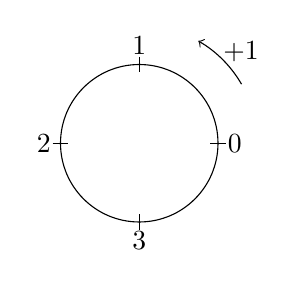
\begin{tikzpicture}
        \tikzset{
            smallline/.pic={
                \draw (0, 1mm) -- (0, -1mm);
            }
        }
        \draw (0, 0) pic[rotate=90] {smallline}
            node[anchor=west] {0}
            arc[radius=1, start angle=0, end angle=90]
            pic {smallline}
            node[anchor=south] {1}
            arc[radius=1, start angle=90, end angle=180]
            pic[rotate=90] {smallline}
            node[anchor=east] {2}
            arc[radius=1, start angle=180, end angle=270]
            pic {smallline}
            node[anchor=north]{3}
            arc[radius=1, start angle=270, end angle=360];

        \draw[->] (0.299, 0.75) arc[radius=1.5, start angle=30, end angle=60]
        node[pos=0.7, anchor=west] {$+1$};
    \end{tikzpicture}
\end{center}
\section{Arithmetic in \texorpdfstring{$\Z_n$}{Zn}}
\begin{propositions}[Arithmetic in $\Z_n$]{
        Let $\congruence{a}{a'}{n}$ and $\congruence{b}{b'}{n}$.
        \label{propArithmeticZn}
    }
    \item $\congruence{a + b}{a' + b'}{n}$ \label{propAdditionZn}
    \item $\congruence{a b}{a' b'}{n}$ \label{propMultZn}
\end{propositions}
\begin{proof}
    Note that we have $n | (a - a')$ and $n | (b - b')$
    \begin{enumerate}
        \item Addition mod $n$:
        We have $n | (a - a' + b - b')$. That is, $n | ((a+b) - (a' + b'))$. So $\congruence{a + b}{a' + b'}{n}$.
        \item Multiplication mod $n$:
        We have $n | (a - a')b$ and $n | (b - b')a'$, so combining these: $n | \left((a - a')b + (b - b')a'\right)$\par
        That is, $n | (ab - a'b')$, so $\congruence{ab}{a'b'}{n}$.
    \end{enumerate}
\end{proof}
So we have that congruences respect addition and multiplication, so we have all of the usual arithmetical operations (except division - see the next section).
\section{Solving Congruences}
We have the usual rules of arithmetic, so we consider what an \textit{equation} looks like in $\Z_n$. 
\begin{example}
    We consider the congruence:
    \begin{equation}
        \congruence{7x}{2}{10}
        \label{eqnSimpleCongruenceExample}
    \end{equation}
    We do not actually have a good idea of what division looks like yet, but we can use multiplication. Note that $\congruence{7 \times 3 = 21}{1}{10}$. Therefore, if we multiply equation~\ref{eqnSimpleCongruenceExample} by 3, we can remove the 7 multiplying $x$:
    \begin{align*}
        &\congruence{3 \times 7x}{3 \times 2}{10} \\
        &\congruence{x}{6}{10}
    \end{align*}
    And this is what a solution looks like in $\Z_n$ - the solutions are unique up to congruence.
\end{example}
\begin{definition}{Modular inverse}
    Given $a, b \in \Z_n$, we say that $b$ is an \underline{inverse} of $a$ if $\congruence{a \times b}{1}{n}$. If such a $b$ exists, we say that $a$ is \underline{invertible} or a \underline{unit} mod $n$. We write $a^{-1}$ for this inverse, if it exists.
\end{definition}
\begin{proposition}
    Inverses are unique modulo $n$.
\end{proposition}
\begin{proof}
    Suppose there exists integers $b$ and $b'$ such that $\congruence{ab}{1}{n}$ and $\congruence{ab'}{1}{n}$.\par
    \begin{align*}
        b &\equiv (ab')b \\
        &\equiv b'(ab) \\
        &\equiv b'
    \end{align*}
    So $\equiv{b}{b'}{n}$. That is, any two inverses must be congruent to each other.
\end{proof}
Now we have some form of division or cancellation in modulo arithmetic: if $a$ is a unit, then we can say $\congruence{ab}{ac}{n} \implies \congruence{b}{c}{n}$.
\begin{proposition}
    Let $n \geq 2$. $a$ is a unit mod $n$ if and only if $a$ and $n$ are coprime.
    \label{propUnitsCoprimes}
\end{proposition}
\begin{proof}
    We have $\hcf{(a, n)} = 1$, so by theorem~\ref{thmLinearComboHCF}, we have some integers $x$ and $y$ such that $ax + ny = 1$.\par
    This is equivalent to $ax = 1 - ny$, or $\congruence{ax}{1}{n}$, and we note that $x$ is the inverse of $a$.
\end{proof}
\begin{corollary}
    For $a$ and $n$ coprime, the congruence $\congruence{ax}{b}{n}$ has a unique solution.
    \label{corCongruenceSolutions}
\end{corollary}
We end up with a similar result to \ref{thmBezout} for congruences of the form
\begin{equation}
    \congruence{ax}{b}{n}, \text{ where } \hcf{(a, n)} = d > 1
    \label{eqnHCFCongruence}
\end{equation}
We then find that there is a solution if and only if $d | b$. In this case, dividing equation~\ref{eqnHCFCongruence} by $d$ gives an equation of the form discussed in corollary~\ref{corCongruenceSolutions}.
\section{Simulataneous congruences}
In order to solve simultaneous congruences, we need an important theorem.
\begin{theorem}[Chinese Remainder Theorem]
    Let $m$ and $n$ be coprime. Let $a, b \in \Z$.\par
    Then there is a unique solution to the simultaneous congruences:
    \begin{align*}
        &\congruence{x}{a}{m} \\
        &\congruence{x}{b}{n} \\
    \end{align*}
    that is unique modulo $mn$.
    \label{thmChineseRemainder}
\end{theorem}
\begin{proof}
    We first find a solution.\par
    Since $m$ and $n$ are coprime, we have $s m + t n = 1$ for some integers $s$ and $t$. Therefore, $\congruence{sm}{1}{m}$ and $\congruence{tn}{1}{m}$.\par
    Now consider the linear combination $x = a(tn) + b(sm)$. Then we have:
    \begin{align*}
        &\congruence{x}{a + 0}{m} \\
        &\congruence{x}{b + 0}{n} 
    \end{align*}
    So $x$ solves the simultaneous congruences.\par
    We then show this solution is unique.\par
    Suppose $y$ is also a solution, so $\congruence{y}{a \equiv x}{m}$ and $\congruence{y}{b \equiv x}{m}$.\par
    Then:
    \begin{align*}
        &\implies m | (y - x) \text{ and } n | (y - x) \\
        &\implies mn | (y - x) \text{ since } \hcf{(m, n)} = 1 \\
        &\implies \congruence{y}{x}{mn}
    \end{align*}
\end{proof}
\begin{remark}
    Theorem~\ref{thmChineseRemainder} can also be extended by induction to systems of more than 2 simultaneous congruences.
\end{remark}
\section{More on Exponentiation in \texorpdfstring{$\Z_n$}{Zn}}
We first introduce a very interesting function that can simplify theorems relating to exponentiation in $\Z_n$.
\begin{definition}{Euler totient function}
    For a natural number $n$, denote the number of integers $a$ with $1 \leq a \leq n$ that are coprime with $n$ as $\varphi(n)$. The function $\varphi$ is the \underline{Euler totient function}.
\end{definition}
Note that $\varphi(1)$ is 1.\par
If $p$ is a prime, $\varphi(p) = p - 1$. If, further, $q$ is a prime, then $\varphi(pq) = pq - p - q + 1$.
\begin{example}
    What are the powers of 2 mod 7?\par
    \begin{equation*}
        2^1 \equiv 2, 2^2 \equiv 4, 2^3 \equiv 1, 2^4 \equiv 2, \cdots
    \end{equation*}
\end{example}
We can introduce some theorems to make this process easier.
\begin{theorem}[Fermat's Little Theorem]
    Let $p$ be prime. Then $\congruence{a^p}{a}{p}$.
    \label{thmFermatLittle}
\end{theorem}
The theorem is alternately stated $\congruence{a^{p-1}}{1}{p}$ if $a \neq 0$.
\begin{proof}
    If $a = 0$ then we are done.\par
    If $a \neq 0$ then $a$ is a unit mod $p$ by proposition~\ref{propUnitsCoprimes}. Therefore, $\congruence{ax}{ay}{p}$ if and only if $\congruence{x}{y}{p}$. Hence the numbers
    \begin{equation*}
        a, 2a, \cdots, (p-1)a
    \end{equation*}
    are pairwise incongruent and non-zero. Therefore, they must be some permutation of $\{1, 2, \cdots, p-1\}$. Then consider their product:
    \begin{align*}
        (a)(2a)\cdots((p-1)a) &\equiv (1)(2)\cdots(p-1)\text{ mod } p \\
        a^{p-1}(p-1)! &\equiv (p-1)! \\
        a^{p-1} &\equiv 1 \text{ since all integers are units.}
    \end{align*}
\end{proof}
We can also extend this to non-prime elements by requiring coprimality.
\begin{theorem}[Euler-Fermat Theorem]
    \label{thmEulerFermat}
    Let $a$ and $m$ be coprime integers. Then $\congruence{a^{\varphi(m)}}{1}{m}$.
\end{theorem}
\begin{proof}
    Let $U$ be the set of units:
    \begin{equation*}
        U = \subsetselect{x \in \Z}{0 < x < m, \hcf{(x, m)} = 1}
    \end{equation*}
    And label each element $u_1, \cdots, u_{\varphi(m)}$.\par
    Then $a u_1, a u_2, \cdots, a u_{\varphi(m)}$ are all distinct and invertible mod $m$ since $a$ is a unit (by assumption). They are thus congruent to the elements of $U$ after permutation. Consider their product:
    \begin{align*}
        \prod_{u \in U} a u &\equiv \prod_{u \in U} u \\
        a^{\varphi(m)} \prod_{u \in U} u &\equiv \prod_{u \in U} u
    \end{align*}
    But a product of units is invertible:
    \begin{equation*}
        \congruence{a^{\varphi(m)}}{1}{m}
    \end{equation*}
\end{proof}
The proof of Fermat's little theorem involved the number $(p-1)!$. We can introduce a theorem to tell us more about this number, mod p, but first we need to think about squares mod $p$.
\begin{lemma}
    Let $p$ be prime. Then $\congruence{x^2}{1}{p}$ if and only if $x \equiv 1$ or $x \equiv -1$ mod $p$.
    \label{lemSqrt1ModP}
\end{lemma}
\begin{proof}
    \begin{proofdirection}{$\Rightarrow$}{Assume $\congruence{x^2}{1}{p}$}
        Note that $\congruence{x^2}{1}{p}$ is equivalent to $p | (x^2 - 1)$.\par
        Therefore we can factorise:
        \begin{equation*}
            p | (x + 1)(x - 1)
        \end{equation*}
        And since $p$ is prime we can use proposition~\ref{propPrimeDivisibility} to get that $p$ divides $x+1$ or $x-1$. That is, $\congruence{x}{1}{p}$ or $\congruence{x}{-1}{p}$.
    \end{proofdirection}
    The backward direction is trivial: $x = \pm 1 \implies x^2 = 1$ as required.
\end{proof}
Now we can think about $(p-1)!$.
\begin{theorem}[Wilson/Al-Haytham Theorem]
    Let $p$ be prime. Then $\congruence{(p-1)!}{-1}{p}$.
    \label{thmFactorialPMinusOne}
\end{theorem}
\begin{proof}
    We have the trivial case $p = 2$ holds ($\congruence{1! = 1}{-1}{p}$), so consider only odd primes.\par
    All of the multiplied numbers in $(p-1)!$ are either self-inverse or not self inverse. The elements that are not self-inverse will therefore cancel out with their inverse, leaving only a product of terms that are not self-inverse. A self-inverse element must square to 1 by definition, so by lemma~\ref{lemSqrt1ModP} these elements are $1$ and $-1$.\par
    Therefore we group all numbers that are not self-inverse into pairs, leaving only the self-inverse elements $1$ and $-1$. The product of all of this is therefore $-1$.
\end{proof}
We now know how to solve $\congruence{x^2}{1}{p}$. But what about the similar congruence $\congruence{x^2}{-1}{p}$?
\begin{proposition}
    Let $p$ be an odd prime. Then $-1$ is a square mod $p$ if and only if $\congruence{p}{1}{4}$.\label{propMinusOneModP}
\end{proposition}
\begin{proof}
    \begin{proofdirection}{$\Rightarrow$}{Assume $\congruence{p}{1}{4}$.}
        By theorem~\ref{thmFactorialPMinusOne}, we have:
        \begin{align*}
            -1 &\equiv (p-1)! \text{ mod } p \\
            &\equiv 1 \times 2 \times \cdots \times \frac{p-1}{2} \times \frac{p+1}{2} \times \cdots \times (p-2) \times (p-1) \\
            &\equiv (-1)^{\frac{p-1}{2}} \times \left(\left(\frac{p-1}{2}\right)!\right)^2
        \end{align*}
        And since $\congruence{p}{1}{4}$, let $p = 4k + 1$. Then:
        \begin{align*}
            -1 &\equiv (-1)^{2k} \times \left(\left(\frac{p-1}{2}\right)!\right)^2 \\
            &\equiv \left((-1)^k \left(\frac{p-1}{2}\right)!\right)^2
        \end{align*}
        Which is a square number, as required.
    \end{proofdirection}
    \begin{proofdirection}{$\Leftarrow$}{Assume $\congruence{x^2}{-1}{p}$.}
        Assume for contradiction that $\congruence{p}{3}{4}$, and $p$ can be written $4k + 3$.\par
        Then by theorem~\ref{thmFermatLittle}, $\congruence{x^{p-1}}{1}{p}$.
        \begin{align*}
            1 &\equiv x^{4k+2} \text{ mod } p \\
            &\equiv \left(x^2\right)^{2k+1} \\
            &\equiv (-1)^{2k+1} \\
            &\equiv -1
        \end{align*}
        But $p \neq 2$ so $1 \not\equiv -1$. \contradiction\par
        So $p$ must be congruent to $1$ mod $4$.
    \end{proofdirection}
\end{proof}
\begin{remark}
    This proof gives the solution to the congruence $\congruence{x^2}{-1}{p}$ in the case $\congruence{p}{1}{4}$.
\end{remark}
\nonexaminablesection{\texorpdfstring{$\Z_p$}{Zp} as a group under multiplication}
\section{Asymmetric Encryption}
An important application of modulo arithmetic is in cryptography. In the 1970s at the dawn of the internet it became increasingly important that communications could be sent securely and, if intercepted, could not be read. Therefore mathematicians wondered how to create a cryptographical system in which it is impossible to decrypt a message without the \textit{key}, but without requiring this key to be transmitted between the two parties.
The first example of an asymmetrical encryption scheme (in which a different key is used for encryption as decryption) was RSA, named after its creators Rivest, Shamir and Alderman.
\begin{enumerate}
    \item Begin by choosing two very large prime numbers $p$ and $q$
    \item Compute their product $n$, and choose a number $e$ which is coprime to $\varphi(n)$ - this is the \textit{encoding exponent}
    \item Publish the pair $(n, e)$ - this is the \textit{public key}
    \item To send an encrypted message, split it into packets, $M$ where $M < n$
    \item Send $M^e$ mod $n$, using squaring to achieve more efficient exponentiation
    \item The receiver then calculates the \textit{decoding exponent} to be the smallest integer $d$ such that $\congruence{de}{1}{\phi(n)}$
    \item The receiver computes $\left(M^e\right)^d$, which is congruent to $M$ mod $n$ by theorem~\ref{thmEulerFermat}.
\end{enumerate}
Anyone wishing to read the message therefore must know:
\begin{itemize}
    \item $n$, which is published
    \item $e$, which is published
    \item $\varphi(n)$, which, for sufficiently large choices of $p$ and $q$, is unfeasible since it requries factoring $n$.
\end{itemize}
\end{document}